\section{Introduction}

The human brain is a spatiotemporal dynamic system whose activity can be non-invasively measured using functional magnetic resonance imaging (fMRI). 
A large body of work has leveraged fMRI to investigate functional connectivity patterns for tasks such as neurological disorder diagnosis or demographic attribute prediction \citep{BNC, BNT, meanmlp, TFF, swift, brainlm, brainjepa}. 
Existing approaches can be broadly divided into two categories: ROI-based methods and voxel-based methods.  
\begin{figure}
  \centering
  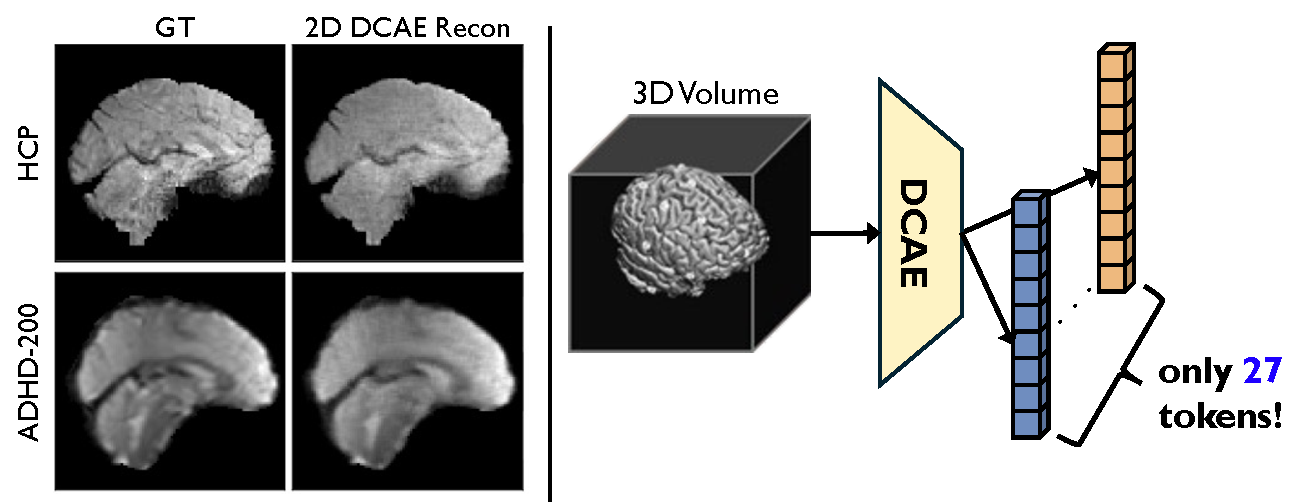
\includegraphics[width=\linewidth]{figures/tablet_teaser.pdf}
  \caption{We show that a 2D natural image autoencoder can be transferred well to 4D fMRI data (left). Building on this, we propose to tokenize a single 3D volume of fMRI only into 27 tokens, enabling longer spatiotemporal modeling with a simple Transformer architecture (right).}
  \label{fig:teaser}
  \vspace{-5mm}
\end{figure}
ROI-based methods first define a set of regions of interest (ROIs) based on anatomical segmentation \citep{FC}, extract their corresponding time-series signals, and then compute functional connectivity (FC) matrices as model inputs.
Although this approach is computationally efficient for managing the high dimensionality of fMRI data, it has several limitations: performance strongly depends on the choice of ROIs, fine-grained 3D spatial structures may be lost, and aggressive compression can discard informative signals. 
To overcome these limitations, voxel-based methods such as TFF~\citep{TFF} and SwiFT~\citep{swift} have been proposed. These methods directly process raw 4D fMRI data, thereby preserving spatial and temporal information, while also allowing detailed interpretation as they directly operate on the given image. 
However, due to the massive scale of fMRI volumes, the temporal length that could be simultaneously processed by the model is severely restricted (e.g., TFF and SwiFT use only 20 timesteps at once), potentially missing informative long-range temporal dynamics, and limiting use for tasks that require longer-range interactions, such as the infraslow BOLD–LFP coupling and global arousal waves that unfold over tens of seconds~\citep{pan2013infraslow,raut2021global}.

In this work, we aim to improve voxel-based fMRI modeling by \emph{tokenizing} fMRI volumes into a compact set of continuous tokens, thereby enabling Transformers \citep{attention} to process substantially longer temporal sequences. 
To this end, we observed a strong perceptual information preservation capability of the Deep Compression Autoencoder (DCAE)~\citep{DCAE} and aimed to leverage it, as it effectively tokenizes a \(256 \times 256\) 2D natural image into just 64 continuous tokens (a compression ratio of 32). 
Motivated by this, we ask whether a high-performing \textit{\textbf{2D}} autoencoder trained on \textit{\textbf{natural images}} can serve as an effective tokenizer for \textit{\textbf{4D fMRI}} data. 

Although it may seem counterintuitive, we demonstrate that such an autoencoder can effectively tokenize fMRI volumes while preserving both fine-grained and high-level functional information.
Namely, by rearranging the tokens extracted from each 2D slice of a 3D fMRI volume, we compress an entire volume into \textit{only} 27 continuous tokens, thereby dramatically reducing the input size and enabling substantially longer-sequence modeling with a simple Transformer encoder-based architecture even with limited VRAM. We dub our method {\ours}, \textbf{T}wo-dimensionally \textbf{A}utoencoded \textbf{B}rain \textbf{L}at\textbf{e}nt \textbf{T}ransformer, which achieves consistent yet modest improvements compared to voxel-based baselines on demographic attribute prediction and attention-deficit hyperactivity disorder (ADHD) diagnosis tasks. 

Our model drastically saves memory and computation costs compared to the most efficient voxel-based baseline under the same input data scale, allowing much longer sequences to be fed into the model. This unlocks the opportunity for future use cases that require such long sequences.
Moreover, we demonstrate that self-supervised masked token modeling on fMRI data can effectively pre-train the model, thereby improving downstream task performance.


Our core contributions are summarized as follows:

\begin{compactitem}
\item We propose a novel tokenization scheme that utilizes a 2D autoencoder, which is pre-trained on natural images. We then empirically demonstrate that, despite the apparent domain mismatch, it can serve as a practical general-purpose tokenizer for fMRI signals.
\item Building on this tokenization, we construct a simple Transformer architecture to model substantially longer temporal sequences than prior state-of-the-art voxel-based models, leading to performance improvements across multiple tasks based on resting-state fMRI (rs-fMRI) datasets. This approach would allow application to tasks that require longer-range interactions.
\item Furthermore, we show the feasibility of pre-training on tokenized fMRI data using self-supervised masked token modeling, which can further improve downstream task performance.
\end{compactitem}



